\section*{Abstract}
In the dynamic realm of wireless communication, the pursuit of efficient and dependable antennas operating at high frequencies has emerged as a pivotal endeavor. This project embarks on a comprehensive exploration of the intricacies involved in implementing an oscillator finely tuned for integration into an antenna system operating at approximately 3.5 GHz. By interfacing with a matching network, this oscillator aims to augment the functionality of the transmitter antenna. The paramount significance of this undertaking stems from its potential to propel the performance benchmarks of communication systems, thereby aligning with the constantly evolving landscape of modern connectivity.\par
At its core, this project delves into the interdisciplinary domain encompassing Radio Frequency (RF) engineering, Microwave engineering, and Analog Integrated Circuits. The realization of RF systems, particularly those operating at challenging frequencies around 3.5 GHz, necessitates a nuanced comprehension of various domains including circuit theory, analog circuits, frequency response, electromagnetic principles, and communication systems. The amalgamation of these disciplines forms the bedrock upon which the project endeavors to advance the frontier of wireless communication technology.\par

\begin{figure}[!h]
    \centering
    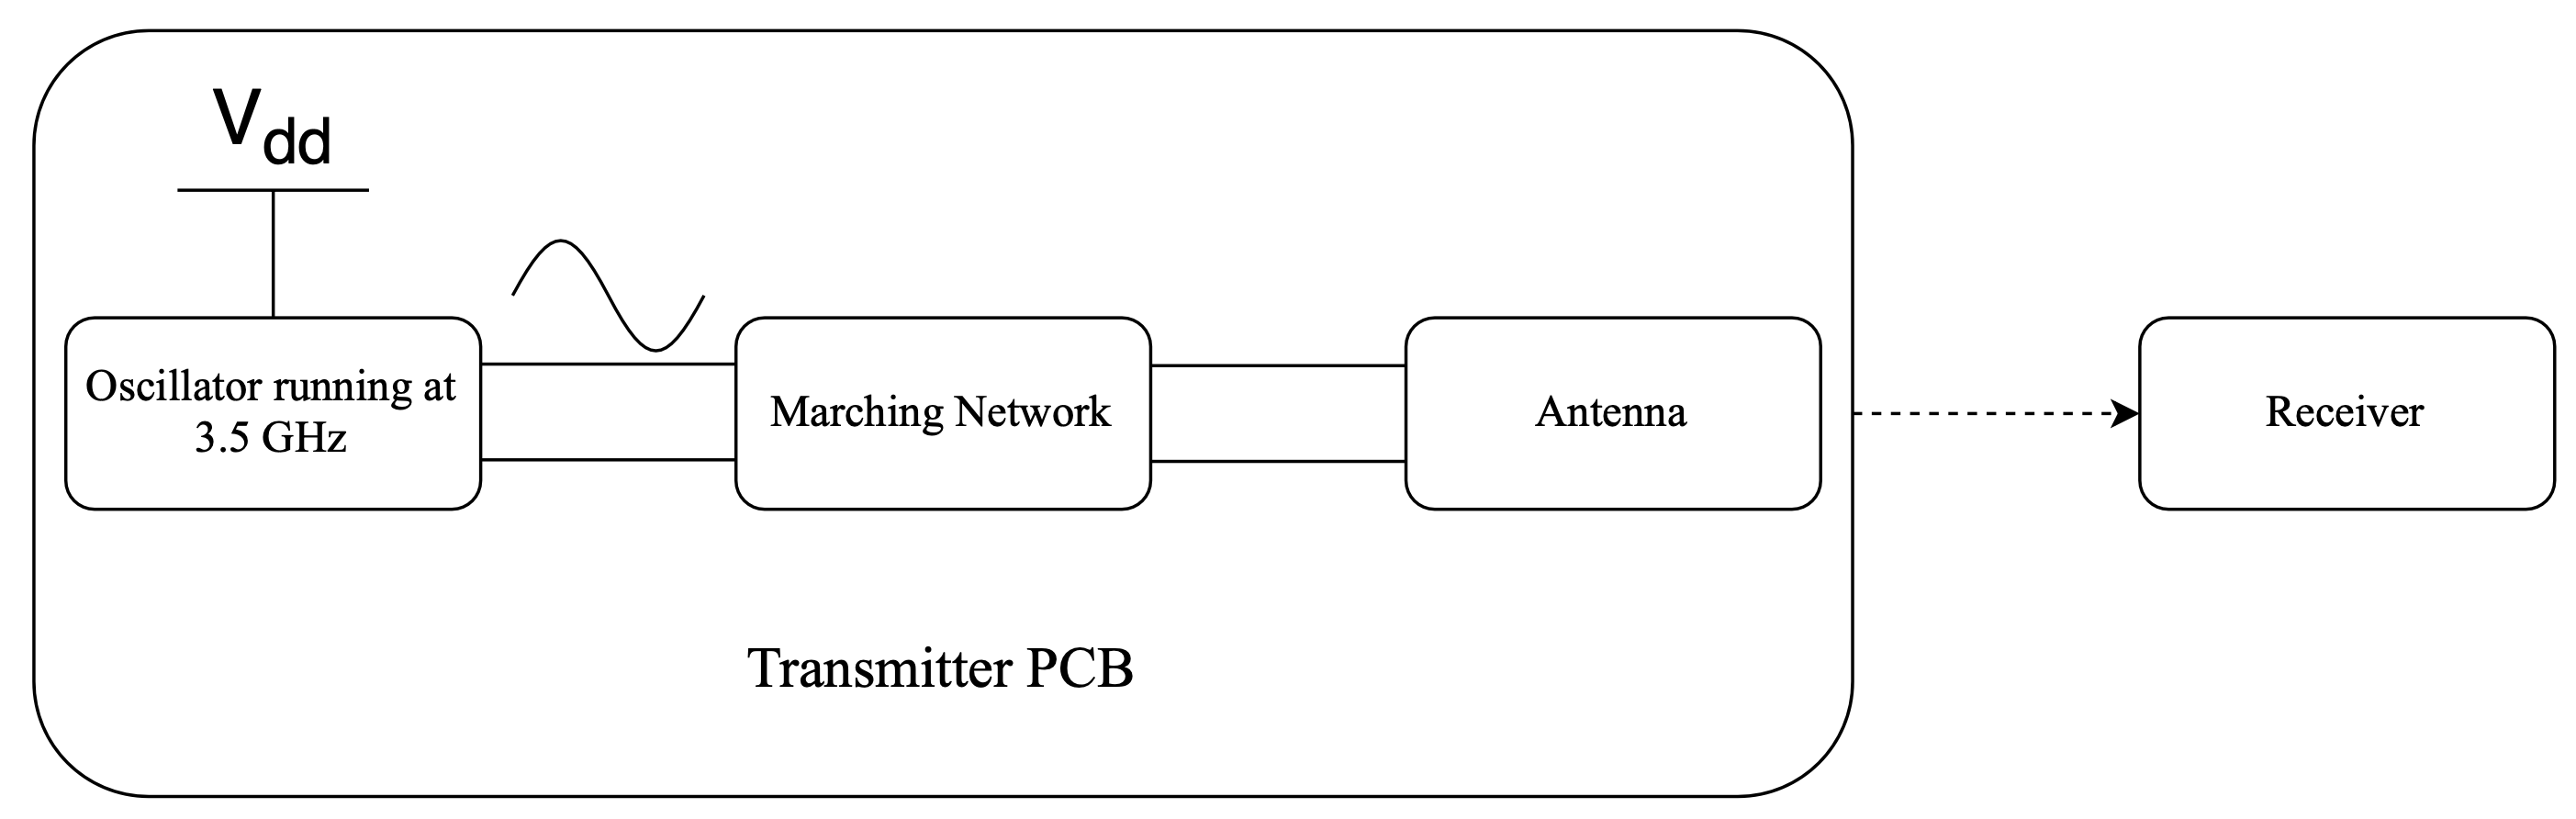
\includegraphics[width=0.8\linewidth]{images/misc/block_diagram.png}
    \caption{Block Diagram}
    \label{fig:block-diagram}
\end{figure}

Oscillators, owing to their intrinsic capability to generate stable and precise periodic waveforms, find extensive utility across a myriad of applications. The envisioned 3.5 GHz high-frequency oscillator, poised for development in this project, holds promise in realms ranging from 5G networks to satellite communication systems. Moreover, the utility extends to radar systems for navigation, RFID tags utilized in smartcards, and the intricate realm of Magnetic Resonance Imaging (MRI). This underscores the multifaceted impact that the successful realization of such an oscillator could wield across diverse industries, transcending mere advancements in antenna systems to usher in efficiency, precision, and reliability across a spectrum of technological applications.\par

Central to the project's endeavor is a meticulously structured implementation plan, delineated into several distinct phases. The initial phase entails the construction of an oscillator model, a pivotal step that sets the foundation for subsequent developments. Through the utilization of Spice simulation, this phase aims to validate the efficacy of the oscillator model at the targeted frequency of 3.5 GHz. Subsequently, the project pivots towards the selection of appropriate components, a process encompassing the careful identification of the optimal transistor—be it an NPN BJT or an NMOS—capable of operating within the designated frequency range. This necessitates the creation and validation of a corresponding spice model, which is subsequently subjected to simulation using Cadence Virtuoso to ascertain S-parameters.\par

The integration of the oscillator with the transmitter antenna necessitates meticulous attention to antenna matching—a process crucial for optimizing power transfer and minimizing signal reflections. The intricate interplay between the oscillator and the antenna, facilitated by the matching network, underscores the project's commitment to realizing seamless integration within the broader communication ecosystem. Furthermore, the project envisages the creation of a compact and meticulously optimized Printed Circuit Board (PCB) layout, meticulously designed to mitigate parasitic elements and minimize signal loss—a pivotal consideration in the realm of RF design.\par

The culmination of these meticulously orchestrated phases culminates in a rigorous testing regimen, aimed at validating the integrity and efficacy of the developed oscillator. Through the utilization of a pre-built receiver, the performance of the oscillator is meticulously scrutinized, with particular emphasis placed on parameters such as stability, frequency accuracy, and signal fidelity. This comprehensive testing phase serves as the litmus test for the viability and functionality of the developed oscillator, affirming its readiness for integration within real-world communication systems.\par

In conclusion, the project encapsulates a holistic exploration of the intricacies involved in the development of a high-performance 3.5 GHz oscillator, poised to enhance the efficacy and reliability of communication systems operating within this frequency band. Through a meticulous amalgamation of theoretical insights, simulation-based validation, and real-world testing, the project aspires to not only advance the frontier of antenna systems but also foster a broader paradigm shift towards enhanced efficiency, precision, and reliability across diverse technological applications.